\section{Background and Motivation}\label{sec:motivation}

In this section, we explain why traditional graph coverage may not
produce high-quality conformance tests by using JavaScript
as an example language. We select JavaScript because its
mechanized specifications are actively maintained,
while most mechanized specifications of other languages are outdated.
Since all the existing JavaScript mechanized specifications~\cite{kjs, javert, jiset,
skel-js} closely capture the abstract algorithms in ECMA-262~\cite{es13},
we show how the JavaScript mechanized specification 
describes the JavaScript syntax and semantics using ECMA-262.
Then, we explain the control-flow graph (CFG) of abstract algorithms in ECMA-262
and how to use the CFG in coverage-guided fuzzing.
Finally, we demonstrate why a simple node coverage criterion cannot fully
discriminate different semantics in different language features or even in the
same language feature.

%----------------------------------------%
%----------------------------------------%

\subsection{JavaScript Language Specification (ECMA-262)}\label{sec:ecma-262}

Now, we explain how the latest version of ECAM-262 (ES13, 2022) describes
the syntax and semantics of JavaScript language features with simple examples.

%----------------------------------------%
%----------------------------------------%

\subsubsection{Syntax}\label{sec:syntax}

\begin{figure}
  \centering
  \begin{subfigure}{\textwidth}
    \[
      \small
      \begin{array}{l}
        \esntp{AdditiveExpression}{Yield, Await} \est{:}\\

        \qquad \esntp{MultiplicativeExpression}{?Yield, ?Await}\\

        \qquad \esntp{AdditiveExpression}{?Yield, ?Await} \; \est{+} \;
        \esntp{MultiplicativeExpression}{?Yield, ?Await}\\

        \qquad \esntp{AdditiveExpression}{?Yield, ?Await} \; \est{-} \;
        \esntp{MultiplicativeExpression}{?Yield, ?Await}\\
      \end{array}
    \]
  \end{subfigure}
\vspace*{-.5em}
  \caption{Syntax of \esnt{AdditiveExpression} in ES13}
\vspace*{-.5em}
  \label{fig:add-syntax}
\end{figure}

ECMA-262 defines JavaScript syntax with a variant of the extended Backus–Naur form (EBNF).
It consists of syntactic productions defined with multiple alternatives;
each alternative is a sequence of symbols.
Unlike the original EBNF, its nonterminals are parametric with boolean arguments:
$\esparam{?}$ denotes passing the argument as is, and $\esparam{+}$
and $\esparam{\(\sim\)}$ denote passing \scode{true} and \scode{false}, respectively.
In addition, it supports various extensions, including
context-sensitive symbols and conditional alternatives.
For example, consider the following simple additive expression:
\begin{equation}\label{equ:add}
  \jscode{1 + 2}
\end{equation}
It computes the addition of two Number values, \jscode{1} and
\jscode{2}.
Figure~\ref{fig:add-syntax} describes its syntax with the production of \esnt{AdditiveExpression}\footnote{
\url{https://262.ecma-international.org/13.0/\#prod-AdditiveExpression}}.
It requires two boolean parameters, \esparam{Yield} and \esparam{Await}, and
consists of three alternatives.
The second (or third) alternative consists of three symbols: a nonterminal
\esnt{AdditiveExpression}, a terminal \est{+} (or \est{-}), and a nonterminal
\esnt{MultiplicativeExpression}.

%----------------------------------------%
%----------------------------------------%

\subsubsection{Semantics}\label{sec:sem}

\begin{figure}
  \centering
  \begin{subfigure}{\textwidth}
    \small
    %----------------------------------------%
    $\fbox{\textsf{Syntax-directed operations (SDOs)}}$
    \vspace*{0.5em}\\
    %----------------------------------------%
    \textbf{Evaluation} of
    \esnt{AdditiveExpression} \est{:} \esnt{AdditiveExpression} \est{+}
    \esnt{MultiplicativeExpression}
    \\
    \null\quad 1. Return ?$\lab{2}$
    \esalg{EvaluateStringOrNumericBinaryExpression}$\lab{1}$(\esnt{AdditiveExpression},
    \escode{+}, \esnt{MultiplicativeExpression}).$\lab{3}$
    \vspace*{0.5em}\\
    %----------------------------------------%
    \textbf{Evaluation} of
    \esnt{AdditiveExpression} \est{:} \esnt{AdditiveExpression} \est{-}
    \esnt{MultiplicativeExpression}
    \\
    \null\quad 1. Return ?$\lab{5}$
    \esalg{EvaluateStringOrNumericBinaryExpression}$\lab{4}$(\esnt{AdditiveExpression},
    \escode{-}, \esnt{MultiplicativeExpression}).$\lab{6}$

  \end{subfigure}
\vspace*{-1.5em}
  \caption{
    Semantics of \esnt{AdditiveExpression} defined with two syntax-directed
    operations (SDOs) in ES13
  }
  \label{fig:add-sdo}
\end{figure}

The language specification describes semantics using abstract algorithms, and
there are three kinds of abstract algorithms:
%
\begin{itemize}
  \item Syntax-directed operations (SDOs) (e.g., \textbf{Evaluation} of
    \esnt{AdditiveExpression} \est{:} $\cdots$ in Figure~\ref{fig:add-sdo})

  \item Normal algorithms (e.g., \textbf{ToNumeric} in
    Figure~\ref{fig:normal-algos})

  \item Built-in methods (e.g., \textbf{Number} in
    Figure~\ref{fig:builtin-number})
\end{itemize}

%----------------------------------------%

A \textit{syntax-directed operation (SDO)} defines the semantics of each
alternative in syntactic productions.
It consists of 1) a target alternative, 2) a name, 3) optional parameters, and 4) a body.
Each algorithm body is a pseudo-code consisting of well-organized steps written
in a natural language, English.
For example, two abstract algorithms in Figure~\ref{fig:add-sdo} are SDOs whose
target alternatives are the second and third alternatives of
\esnt{AdditiveExpression} production for addition (\scode{+}) and subtraction
(\scode{-}) operators, respectively.
Their names are \textbf{Evaluation} with no optional parameters, and
the bodies consist of a single step that invokes another normal algorithm
\textbf{EvaluateStringOrNumericBinaryExpression}\footnote{
\url{https://262.ecma-international.org/13.0/\#sec-evaluatestringornumericbinaryexpression}}.
Note that the metavariables \esnt{AdditiveExpression} and
\esnt{MultiplicativeExpression} in these SDOs store \textit{abstract syntax
trees (ASTs)} of the left-hand and right-hand sides of given additive
expressions, respectively.
For instance, if the first SDO in Figure~\ref{fig:add-sdo} takes the additive
expressions in~(\ref{equ:add}), the two metavariables store ASTs of two Number
literals, \jscode{1} and \jscode{2}, respectively.
It means that abstract algorithms in ECMA-262 treat ASTs as values and can
store them in variables or pass them as arguments of other algorithms.
The ``?'' operator is a shorthand for the following sequence of steps to handle control flows:
\vspace*{.5em}\\
{
  \noindent
  \null\qquad 1. If \esvar{argument} is an abrupt completion, return
  \esalg{Completion}(\esvar{argument}).
  \\
  \null\qquad 2. Else if \esvar{argument} is a Completion Record, set
  \esvar{argument} to \esvar{argument}.[[Value]].
}
\vspace*{.5em}\\
where a completion record is \textit{abrupt} when it represents exceptional
control flows, such as \jscode{throw}, \jscode{return}, \jscode{break}, and
\jscode{continue}.
In other words, the ``?'' operator is a branch that checks whether given
values are abrupt completions and directly returns them if so.

%----------------------------------------%

\begin{figure}
  \centering
  \begin{subfigure}{\textwidth}
    \small
    %----------------------------------------%
    $\fbox{\textsf{Normal algorithms}}$
    \vspace*{0.5em}\\
    %----------------------------------------%
    \textbf{EvaluateStringOrNumericBinaryExpression} (
      \esvar{leftOperand},
      \esvar{opText},
      \esvar{rightOperand}
    )
    \\
    \null\quad $\lab{7}$...
    \\
    \null\quad 5. Return ?$\lab{9}$
    \esalg{ApplyStringOrNumericBinaryOperator}$\lab{8}$(\esvar{lval},
    \esvar{opText}, \esvar{rval}).$\lab{10}$
    \vspace*{0.5em}\\
    %----------------------------------------%
    \textbf{ApplyStringOrNumericBinaryOperator} (
      \esvar{lval},
      \esvar{opText},
      \esvar{rval}
    )
    \\
    \null\quad $\lab{11}$...
    \\
    \null\quad 3. Let \esvar{lnum} be ?$\lab{13}$
    \esalg{ToNumeric}$\lab{12}$(\esvar{lval}).
    \\
    \null\quad 4. Let \esvar{rnum} be ?$\lab{15}$
    \esalg{ToNumeric}$\lab{14}$(\esvar{rval}).
    \\
    \null\quad 5. If \esalg{Type}(\esvar{lnum}) is different from
    \esalg{Type}(\esvar{rnum})$\lab{16}$, \cfbox{red}{throw a \esval{TypeError}
    exception.}$\lab{\inred{17}}$
    \\
    \null\quad ...$\lab{18}$
    \vspace*{0.5em}\\
    %----------------------------------------%
    \textbf{ToNumeric} ( \esvar{value} )
    \\
    \null\quad $\lab{19}$...
    \\
    \null\quad 2. If \esalg{Type}(\esvar{primValue}) is BigInt$\lab{20}$,
    \cfbox{red}{return
    \esvar{primValue}.}$\lab{\inred{21}}$
    \\
    \null\quad ...$\lab{22}$
  \end{subfigure}
\vspace*{-1.5em}
  \caption{Three normal algorithms transitively used in the semantics of
  \esnt{AdditiveExpression} in ES13}
  \label{fig:normal-algos}
\end{figure}

\begin{figure}
  \centering
  \begin{subfigure}{\textwidth}
    \small
    %----------------------------------------%
    $\fbox{\textsf{Built-in methods}}$
    \vspace*{0.5em}\\
    %----------------------------------------%
    \textbf{Number} ( \esvar{value} )
    \\
    \null\quad 1. If \esvar{value} is present$\lab{23}$, then
    \\
    \null\quad\quad a. Let \esvar{prim} be ?$\lab{25}$
    \esalg{ToNumeric}$\lab{24}$(\esvar{value}).
    \\
    \null\quad ...$\lab{26}$
  \end{subfigure}
\vspace*{-1.5em}
  \caption{
    Built-in method \textbf{Number} in ES13
  }
  \label{fig:builtin-number}
  \vspace*{-1em}
\end{figure}

A \textit{normal algorithm} is the primary form of an abstract algorithm defined
by its 1) name, 2) parameters, and 3) body.
It is commonly used as a helper function, and multiple normal algorithms are
used when defining the semantics of language features.
Hence, the semantics of different language features often share the same normal
algorithms.
For example, both SDOs in Figure~\ref{fig:add-sdo} invoke the same normal
algorithm \textbf{EvaluateStringOrNumericBinaryExpression} with different second
arguments \escode{+} and \escode{-}, respectively.
Then, it transitively invokes other normal algorithms,
\textbf{ApplyStringOrNumericBinaryOperator}\footnote{
\url{https://262.ecma-international.org/13.0/\#sec-applystringornumericbinaryoperator}
} and \textbf{ToNumeric}\footnote{
\url{https://262.ecma-international.org/13.0/\#sec-tonumeric}
}.
Thus, at least three normal algorithms are shared in the semantics of the
addition and subtraction expressions.

%----------------------------------------%

JavaScript provides diverse built-in APIs as opaque functions, such as
\jscode{Object.getPrototypeOf} and \jscode{Number.prototype.toString}.
A \textit{built-in method} defines the semantics of a built-in API.
For example, Figure~\ref{fig:builtin-number} describes the semantics of the
\jscode{Number}\footnote{
\url{https://262.ecma-international.org/13.0/\#sec-number-objects}
} built-in API.
Since its primary functionality is to convert a given JavaScript value to its
corresponding Number value, it also uses the normal algorithm \textbf{ToNumeric}
as a helper function.

%----------------------------------------%
%----------------------------------------%

\subsubsection{Language Features}\label{sec:feat}

In JavaScript, a language feature is 1) a \textit{syntactic feature} or 2) a
\textit{built-in API feature}.
A syntactic feature is related to a specific JavaScript syntax consisting of an
alternative in a syntactic production and its corresponding SDO.
On the other hand, a built-in API feature is related to a built-in API instead
of a specific syntax.
For example, the \scode{+} and \scode{-} operators are
syntactic features ($\addfeat$ and $\subfeat$) defined by the second and third
alternatives of \esnt{AdditiveExpression} and their corresponding \textbf{Evaluation} SDOs.
The \textbf{Number} built-method describes the semantics of a built-in
\jscode{Number} API feature ($\numfeat$).

\subsection{Control Flow Graph (CFG) of ECMA-262}\label{sec:cfg}

\begin{figure}[t]
  \centering
  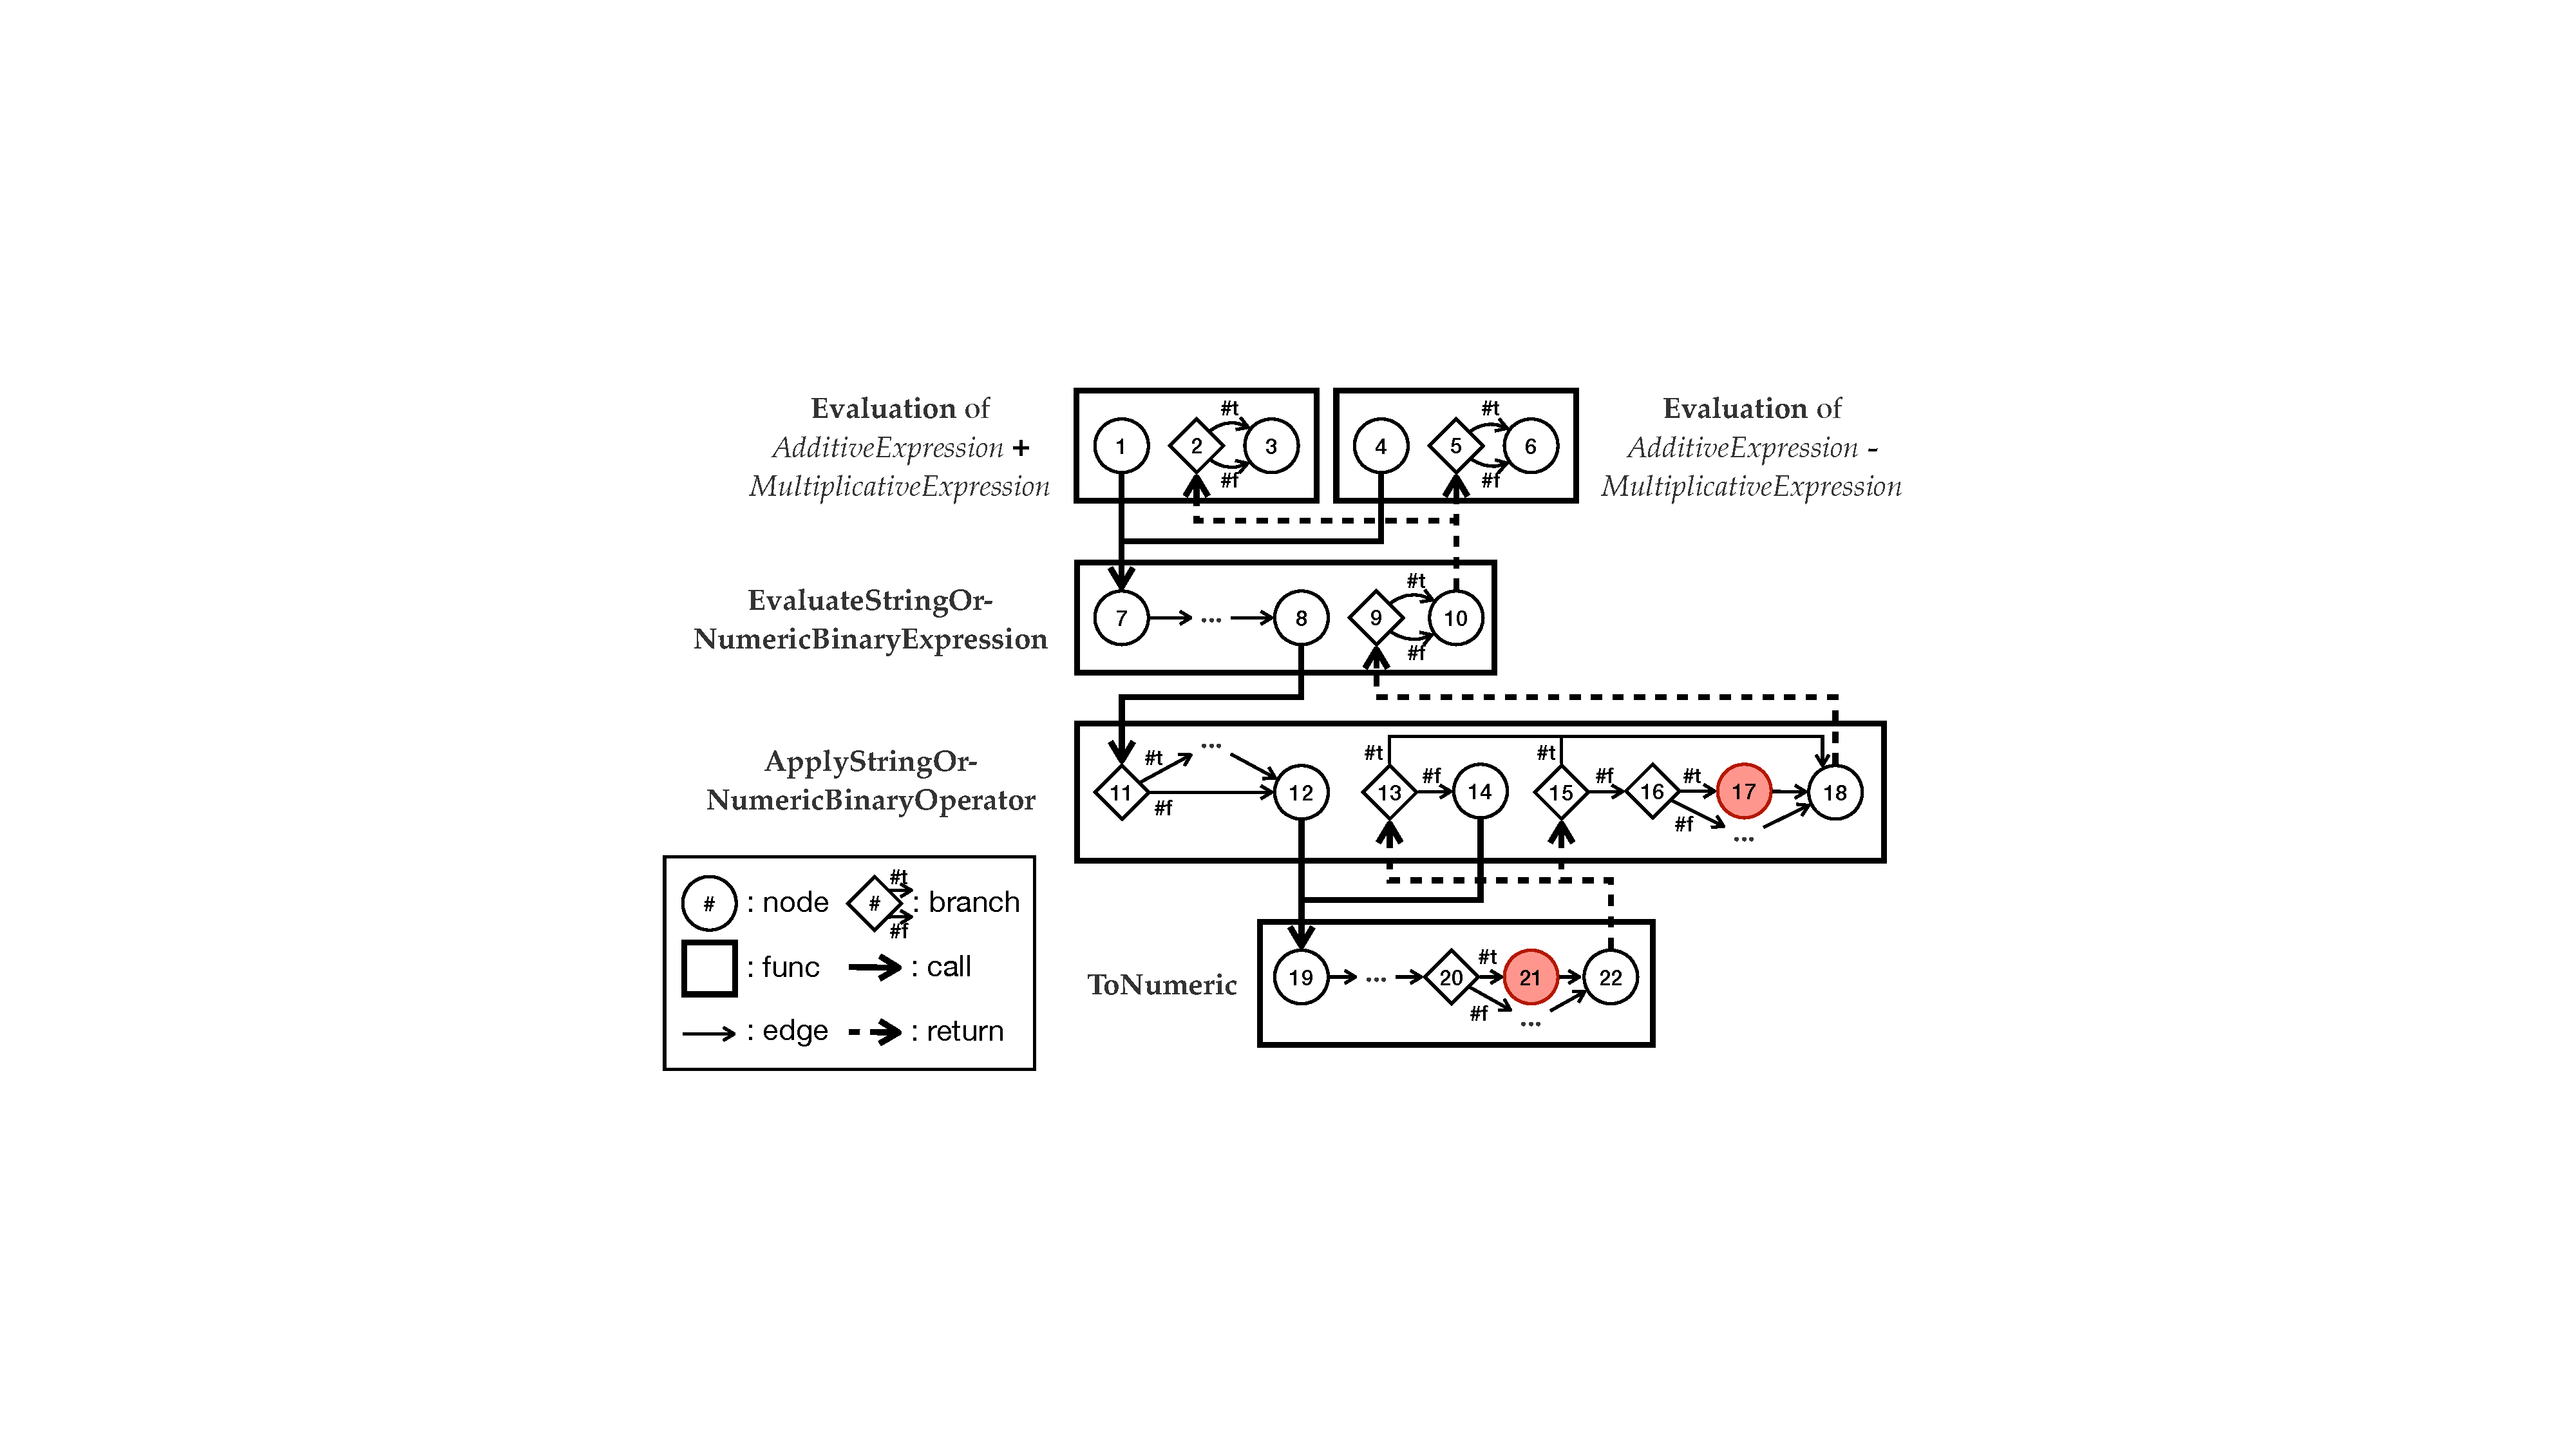
\includegraphics[width=0.87\textwidth]{img/spec-cfg}
  \caption{
    Control-flow graph (CFG) of abstract algorithms in
    Figures~\ref{fig:add-sdo}, \ref{fig:normal-algos}, and
    \ref{fig:builtin-number}
  }
  \label{fig:spec-cfg}
\vspace*{-1em}
\end{figure}

To define the coverage of a conformance test suite using graph coverage criteria,
we need a directed graph of the JavaScript mechanized specification.
CFG is the most common way to construct a directed
graph from a mechanized language specification.
In a CFG, a node denotes a sequence of instructions, and an edge
indicates a control flow in the mechanized specification.
An edge often has an annotation to represent a specific control flow,
such as conditional branches (\sname{\#t} or \sname{\#f}) and function calls
(\sname{call}) and returns (\sname{ret}).

For example, Figure~\ref{fig:spec-cfg} depicts a CFG of the abstract algorithms
in Figures~\ref{fig:add-sdo}, \ref{fig:normal-algos}, and
\ref{fig:builtin-number}.
In this figure, circles (or diamonds) denote nodes (or branches), arrows denote
edges, and boxes indicate algorithms.
The labels inside nodes match the labels annotated in the algorithms in
Figures~\ref{fig:add-sdo},~\ref{fig:normal-algos}, and~\ref{fig:builtin-number}.
Let us apply coverage-guided fuzzing~\cite{afl} with a node coverage
criterion in the CFG and assume that a simple JavaScript program, \jscode{1 + 2},
exists in the program pool.
It does not satisfy the condition in the branch labeled 20 because the left-hand and
right-hand sides of \jscode{1 + 2} are both Number values rather than BigInt values.
Thus, it does not cover the red node labeled 21.
Now assume that another program, \jscode{3n + 4n}, is generated by mutating
the previous program.
Then, it covers the red node labeled 21 because it satisfies the condition
in the branch labeled 20 with BigInt values on both sides of the \jscode{+} operator.

%----------------------------------------%
%----------------------------------------%

\subsection{Motivation}\label{sec:motiv}

Unfortunately, a simple node coverage criterion in CFGs of mechanized
specifications cannot fully discriminate different semantics in different
language features or even in the same feature.
We explain such cases with simple examples using the CFG in Figure~\ref{fig:spec-cfg}.

%----------------------------------------%
%----------------------------------------%

\subsubsection{Different Semantics in Different Language
Features}\label{sec:diff-feat}

The semantics of different language features may use the same abstract
algorithms as helper functions.
For example, the semantics of \scode{+} and \scode{-}
operators transitively use \textbf{ApplyStringOrNumericBinaryOperator}.
In the algorithm, the red node labeled 17 represents throwing
\textbf{TypeError} exception.
If the program pool contains a program \jscode{2n + 1}, it covers the red node
labeled 17 because it has different types of numeric values, a BigInt
\jscode{2n} and a Number \jscode{1}, as the left-hand and right-hand sides of the
\scode{+} operator.
Similarly, another program \jscode{2n - 1} using the \scode{-} operator
covers the node.
However, \jscode{2n - 1} will not be added to the program pool because
the node labeled 17 is already covered by \jscode{2n + 1},
even though \jscode{2n - 1} may reveal a different implementation of the semantics.
For a higher quality of conformance testing,
a more fine-grained definition of graph coverage is necessary
to discriminate \jscode{2n + 1} and \jscode{2n - 1}.

%----------------------------------------%
%----------------------------------------%

\subsubsection{Different Semantics in the Same Language
Feature}\label{sec:same-feat}
In addition, different parts in the semantics of the same language feature
may use the same algorithm more than once.
For example, the semantics of the \scode{+} operator uses
\textbf{ApplyStringOrNumericBinaryOperator}, and it invokes
\textbf{ToNumeric} twice in the nodes labeled 12 and 14.
Now, assume that the current program pool contains a program \jscode{2n + 1} again.
Then, the red node labeled 21 is covered by the program \jscode{2n + 1} because
the left-hand side is a BigInt \jscode{2n}.
It means that another similar program \jscode{1 + 2n} would not be added to the
program pool because the test requirement for a node labeled 21 is already covered
by \jscode{2n + 1}.
However, \jscode{1 + 2n} is also a meaningful test case because it checks the
edge case when the right-hand side of the \scode{+} operator is a BigInt value.

In the remainder of the paper, we formally define a feature-sensitive coverage
criterion and its variants to resolve the problems (Section~\ref{sec:fscov}).
Then, we explain how to implement a conformance test synthesizer with
feature-sensitive coverage criteria in Section~\ref{sec:impl}.
Finally, after evaluating feature-sensitive coverage criteria with
mainstream JavaScript implementations (Section~\ref{sec:eval}),
we discuss related work (Section~\ref{sec:related})
and conclude (Section~\ref{sec:conclusion}).
